\section{The Rust Model}
\thispagestyle{plain} % surpress header on first page

This section follows up on the previous one in the sense that it introduces the model created by \cite{Rust.1987} and presents how NFXP and MPEC can be used to estimate its model parameters. My notation is mainly inspired by the one employed in \cite{Su.Judd.2012}. 

\subsection{The Economic Model}

Rust's model is based on the decision making process of Harold Zurcher who is in charge of a bus fleet and has to decide in each period $t = 0, 1, 2, ...$ whether to replace the engine ($d^i_t=1$) of one or more buses $i = 1, 2, ..., M$ in his fleet or otherwise repair them in a less costly way ($d^i_t=0$). The agent, hence, chooses from the action space $\mathcal{D} = \{0, 1\}$. He bases this choice on two state variables which are the observed cumulative mileage $x^i_t$ of a bus since the last engine replacement and some unobserved (by the econometrician) factor $\epsilon^i_t$. The state of a bus $i$ in period $t$ is therefore fully described by ($x^i_t$, $\epsilon^i_t$) $\in \mathcal{S}$. The agent receives an immediate reward in period $t$ from the chosen replacement decision $d^i_t(x^i_t, \epsilon^i_t)$. The choice in turn affects the possible state space $\mathcal{S'}$ in the period $t+1$ as the cumulative mileage after replacement $x^i_{t+1}$ depends on the choice of $d^i_t$. As the agent is forward looking with a discount factor $\beta \in (0, 1)$ he does not simply maximize the immediate reward but rather the expected discounted utility over an infinite horizon with a higher preference for reward occurring closer to the present. The immediate reward can be characterized in the following way: 

\begin{equation}
	u(x^i_t, d^i_t, \epsilon^i_t; \theta_1, RC) = v(x^i_t, d^i_t; \theta_1, RC) + \epsilon^i_t
\end{equation}

with 

\[v(x^i_t, d^i_t; \theta_1, RC) = \left\{
\begin{array}{lr}
-c(x; \theta_1)  & \mbox{if } d^i_t = 0 \\
-RC -c(0;\theta_1) & \mbox{if } d^i_t = 1
\end{array}
\right.
\]

The immediate reward is hence determined by some operating cost $c(.)$ if regular maintenance as opposed to engine replacement is chosen. It consists of a replacement cost $RC$ and the operating cost after resetting the cumulative mileage to zero if replacement is picked. This shows that The choice of the agent $d^i_t$ depends crucially on the cost parameters $\theta_1$ and $RC$. The timing of events for a single bus in the decision process of Harold Zurcher is depicted in Figure \ref{Figure1} below. 
\vspace{3ex}

\begin{figure}[H]
	\caption{\label{Figure1}Timing of the Decision Model}
	\vspace{2ex}
	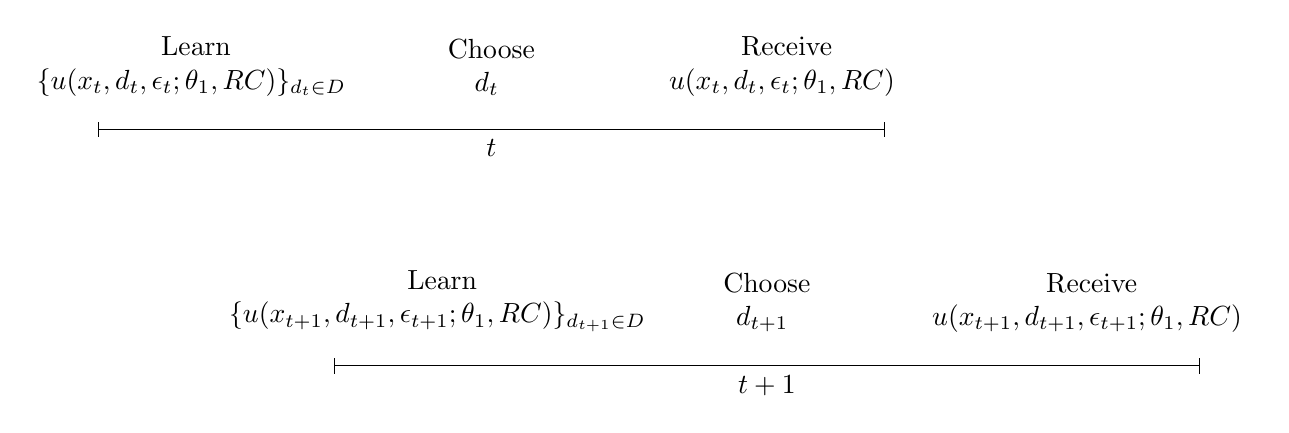
\begin{tikzpicture}
	\draw [|-|]
	(0,1) -- (10,1)
	node [above,align=center,very near start]
	{
		Learn\\
		$\{u(x_t, d_t, \epsilon_t; \theta_1, RC)\}_{d_t \in D}$
		\vspace{2ex}
	}
	node [above,align=center,midway]
	{
		Choose\\
		$d_t$
		\vspace{2ex}
	}
	node [above,align=center,very near end]
	{
		Receive\\
		$u(x_t, d_t, \epsilon_t; \theta_1, RC)$
		\vspace{2ex}
	}
	node [below, align=center, midway]
	{$t$};
	\draw [|-|]
	(3,-2) -- (14,-2)
	node [above,align=center,very near start]
	{
		Learn\\
		$\{u(x_{t+1}, d_{t+1}, \epsilon_{t+1}; \theta_1, RC)\}_{d_{t+1} \in D}$
		\vspace{2ex}
	}
	node [above,align=center,midway]
	{
		Choose\\
		$d_{t+1}$
		\vspace{2ex}
	}
	node [above,align=center,very near end]
	{
		Receive\\
		$u(x_{t+1}, d_{t+1}, \epsilon_{t+1}; \theta_1, RC)$
		\vspace{2ex}
	}
	node [below, align=center, midway]
	{$t+1$};
	
	\end{tikzpicture}
\end{figure}
\vspace{2.5ex}

The transition of the state vector ($x^i_t$, $\epsilon^i_t$) is assumed to follow a Markov process, i.e. the current state only depends on the previous one and hence the utility maximization problem is time-invariant. Dropping the bus index $i$ for convenience, the optimization problem of the agent gives rise to the following value function for a single bus: 

\begin{equation}
V(x_t, \epsilon_t) = \max_{\{d_t, d_{t+1}, ... \}} \E \left[\sum_{\tau=t}^{\infty} \beta^{\tau - t} u(x_\tau, d_\tau, \epsilon_\tau; \theta_1, RC)\right]
\end{equation}

Solving this model leads to an optimal policy rule $\pi^* = (d^{\pi^*}_t(x_t, \epsilon_t))^\infty_t$.

\subsection{The Model Solving}
Given some simplifying assumptions such as conditional independence on the transition probabilities of the state vector, the assumption that the error term $\epsilon_t$ follows a multivariate extreme-value distribution and after discretizing the possible values of the state variable $x$, Rust derives from the original Bellman equation \footnote{The Bellman equation can be found in formula 4.4 on page 1010 in \cite{Rust.1987}} the following contraction mapping needed to solve the economic model:

\begin{equation}
	\label{eq5}
	EV_f(\hat x_k, d) = \sum_{j=0}^{J} log \left\{ \sum_{d'\in\{0, 1\}}  exp[v(x', d'; \theta_1, RC) + \beta EV(x', d')]\right\} \times p_3(x'|\hat x_k, d; \theta_3). 
\end{equation}

with

\[p_3(x'|\hat x_k, d; \theta_3) = \left\{
\begin{array}{lr}
	Pr\{x'=\hat x_{k+j}|\theta_3\}  & \mbox{if } d = 0 \\
	Pr\{x'=\hat x_{1+j}|\theta_3\} & \mbox{if } d = 1
\end{array}
\right.
\]

for $j=0, 1, ..., J$ indicating how many grid points the mileage state climbs up in the next period. \paragraph{}

In the above equation, $EV_f(.)$ denotes the unique fixed point to a contraction mapping $T_f(EV_f, \theta)$ on the full state space $\Gamma_f = \{(\hat x_k, d)|\hat x_k \in \mathbf{\hat x}, d \in \mathcal{D}\}$. Here, $\hat x_k$ represents the grid point $k$ of the state variable $x$ while $\hat x_1 = 0$. The number of possible $\hat x_k$ depends on the choice of the grid size $K$ set by the researcher. The set of possible grid points then is denoted as $\mathbf{\hat x} = \{\hat x_1, ..., \hat x_K\}$. All the variables $v$ depict current period variables while variables $v'$ display the possible value in the next period. The probability $p_3$ indicates how likely it is that a bus moves up a specific amount of grid points in the next period depending on the structural parameter $\theta_3$. Imagine now we decide to set the grid size to $K=90$ as done in \cite{Rust.1987}, then we generally have to find the fixed point above which yields $EV = [EV(\hat x_1, 0), ..., EV(\hat x_{90}, 0), EV(\hat x_1, 1), ..., EV(\hat x_{90}, 1)]$. This simplifies, though, as all the expected values from $EV(\hat x_1, 1), ..., EV(\hat x_{90}, 1)$ are actually equivalent to $EV(\hat x_1, 0)$. This means that in our scenario we just have to find the fixed point for $d=0$, i.e. in our example the vector $EV$ for which we have to actually solve the contraction mapping has a dimension of $90$. This observation will later be important for the difference between NFXP and MPEC. \cite{Su.Judd.2012}, hence, denote the in dimension-reduced contraction mapping shorthand as:

\begin{equation}
EV_r = T_r(EV_r, \theta)
\end{equation}  

with $T_r(.)$ being a contraction mapping on the reduced state space $\Gamma_r = \{(\hat x_k, d=0)|\hat x_k \in \mathbf{\hat x}\}$.

The unique fixed point can now be used to derive conditional choice probabilities of the agent: 

\begin{equation}
	\label{eq7}
	P(d|\hat x; \theta) = \frac{exp[v(\hat x, d; \theta_1, RC) + \beta EV(\hat x, d)]}{\sum_{d' \in \{0, 1\}} exp[v(\hat x, d'; \theta_1, RC) + \beta EV(\hat x, d')]}.
\end{equation}

The above equation describes the probability that the agent chooses $d$ given that the observed mileage state is at a certain grid point $\hat x$. This derivation depends on both the cost parameters ($\theta_1$, $RC$) directly and indirectly through $EV(.)$ on the transition parameter $\theta_3$. These conditional choice probabilities together with the transition probabilities $p_3(.)$ become relevant in the next section when calibrating the model using maximum likelihood. 


\subsection{Calibration}

In order to calibrate the parameter vector $\theta =(\theta_1, \theta_3, RC)$ using either NFXP or MPEC, let us assume that we observe some data set $X = (X^i)^M_{i=1 }$ with $X^i = (x^i_t, d^i_t)^T_{t=1}$ for a single bus $i = 1, ..., M$. The data therefore consists of the engine replacement decision per bus and period as well as the cumulative mileage since the last engine replacement. The cumulative mileage $x^i_t$ is assumed to already be discretized which means that that it takes values on the grid $\mathbf{\hat x} = \{\hat x_1, ..., \hat x_K\}$. The log likelihood of observing the data $X$ now becomes:

\begin{equation}
	L(\theta) = \sum_{i=1}^{M} \sum_{t=2}^{T} log[P(d^i_t|x^i_t; \theta)] + \sum_{i=1}^{M} \sum_{t=2}^{T} log[p_3(x^i_t|x^i_{t-1}, d^i_{t-1}; \theta_3)].
\end{equation}

To fulfill the aim of finding the optimal parameter vector $\theta$ one now has to solve the problem of maximizing the log likelihood:

\begin{equation}
	\max_{\theta} L(\theta).
\end{equation}

The path taken by the NFXP is now to hand this unconstrained optimization problem to an optimization algorithm which comes up with a guess for the optimal parameter $\hat \theta$ for which in a subroutine the expected values in equation \ref{eq5} is calculated for. The expected value function is in turn needed to obtain the conditional choice probabilities in equation \ref{eq7} which are then taken to evaluate the log likelihood $L(\theta)$. Based on this evaluation, the optimization algorithm comes up with a new guess for $\hat \theta$ and the above procedure is repeated until a certain convergence criteria of the algorithm is met. This procedure is again shown in pseudocode in the Algorithm \ref{alg3} on the next page.

At every structural guess of the optimization algorithm the fixed point $EV(.)$ is calculate precisely as it is needed to evaluate the log likelihood $L(\theta)$. This is deemed inefficient by \citeauthor{Su.Judd.2012} which gives rise to the augmented log likelihood mentioned before for which they insert the conditional choice probabilities $P(d^i_t|x^i_t; \theta)$ into $L(\theta)$ making the log likelihood explicitly depend on $EV(.)$. This results in the following log likelihood.

\vspace{2ex}
\begin{algorithm}[!h]
	\caption{Nested Fixed Point Algorithm for the Rust Model}
	\label{alg3}
	\SetAlgoLined
	\KwIn{$\hat\theta_n$, $n=0$, $X$\;}
	\While{$f(|| (\hat\theta_{n+1}, \hat{EV_{n+1}}) - (\hat\theta_{n}, \hat{EV_{n}}) ||) \geq$ stopping tolerance}{
		\vspace{2ex}
		Solve fixed point 	
		\begin{equation*}
		EV(\hat x_k, d) = \sum_{j=0}^{J} log \left\{ \sum_{d'\in\{0, 1\}}  exp[v(x', d'; \hat \theta_{n, 1}, \hat{RC_n}) + \beta EV(x', d')]\right\} \times p_3(x'|\hat x_k, d; \hat \theta_{n, 3});
		\end{equation*}
		
		Given the solution to $EV(.)$ calculate 
		\begin{flalign*}
		P(d|\hat x; \hat \theta_n) = \frac{exp[v(\hat x, d; \hat \theta_{n, 1}, \hat{RC_n}) + \beta EV(\hat x, d)]}{\sum_{d' \in \{0, 1\}} exp[v(\hat x, d'; \hat \theta_{n, 1}, \hat{RC_n})) + \beta EV(\hat x, d')]};
		\end{flalign*}
		
		Evaluate the log likelihood 
		\begin{flalign*}
		L(\hat \theta_n) = \sum_{i=1}^{M} \sum_{t=2}^{T} log[P(d^i_t|x^i_t; \hat \theta_n)] + \sum_{i=1}^{M} \sum_{t=2}^{T} log[p_3(x^i_t|x^i_{t-1}, d^i_{t-1}; \hat \theta_{n, 3})];
		\end{flalign*}
		
		Based on that fix a new guess $\hat\theta_{n+1}$\;
	}
\end{algorithm}
\vspace{2ex}

\begin{equation}
\begin{split}
\mathcal{L}(\theta, EV) = &\sum_{i=1}^{M} \sum_{t=2}^{T} log \left[\frac{exp[v(x^i_t, d^i_t, \theta) + \beta EV(x^i_t, d^i_t)]}{\sum_{d' \in \{0, 1\}}exp[v(x^i_t, d', \theta) + \beta EV(x^i_t, d')]}\right] \\[+3mm]
&+ \sum_{i=1}^{M} \sum_{t=2}^{T} log[p_3(x^i_t|x^i_{t-1}, d^i_{t-1}; \theta_3)]
\end{split}
\end{equation}

In this function nothing guarantees that $\theta$ and $EV$ are actually consistent. This is healed by imposing the fixed point equation \ref{eq5} as constraints to the augmented likelihood function. The MPEC formulation of the calibration problem therefore looks like the following.

\begin{equation}
\begin{aligned}
& \max_{(\theta, EV)} \mathcal{L}(\theta, EV) \\
& \text{subject to } EV = T(EV, \theta).
\end{aligned}
\label{eq2}
\end{equation}

For the MPEC formulation the problem is given to an optimization Algorithm that can handle nonlinear equality constraints. This algorithm then fixes a guess of $(\theta, EV)$ that satisfies the nonlinear constraints, i.e. that is consistent with the underlying economic model and for which the augmented log likelihood is evaluated. Based on this evaluation, the optimizer determines a new guess and the procedure starts over. Again this is done until a specific convergence criteria is met. This procedure is illustrated in algorithm \ref{alg4} on the next page. 


\vspace{2ex}
\begin{algorithm}[!h]
	\caption{MPEC Algorithm for the Rust Model}
	\label{alg4}
	\SetAlgoLined
	\KwIn{$\hat\theta_n$, $\hat{EV_n}$, $n=0$, $X$\;}
	\While{$f(|| \hat\theta_{n+1} - \hat\theta_{n} ||) \geq$ stopping tolerance}{
		\vspace{2ex}
		Evaluate the augmented log likelihood 
		
		\begin{equation*}
		\begin{split}
		\mathcal{L}(\hat\theta_n, \hat{EV_n}) = &\sum_{i=1}^{M} \sum_{t=2}^{T} log \left[\frac{exp[v(x^i_t, d^i_t, \hat\theta_n) + \beta \hat{EV_n}(x^i_t, d^i_t)]}{\sum_{d' \in \{0, 1\}}exp[v(x^i_t, d', \hat\theta_n) + \beta \hat{EV_n}(x^i_t, d')]}\right] \\[+3mm]
		&+ \sum_{i=1}^{M} \sum_{t=2}^{T} log[p_3(x^i_t|x^i_{t-1}, d^i_{t-1}; \hat\theta_{n, 3})]
		\end{split}
		\end{equation*}
		
		Based on that fix a new guess $(\hat\theta_{n+1}, \hat{EV}_{n+1})$\;
	}
\end{algorithm}
\vspace{2ex}

Having established both NFXP and MPEC for the Rust model, let us now turn to some particularities of the model that might be important for the performance of the two algorithms. First of all, \cite{Rust.1987} and \cite{Su.Judd.2012} show that both the likelihood for the NFXP and the MPEC are smooth and their first and second order derivatives exist. In the case of the NFXP this means that Newton's method can be used for the maximization problem. This further helps modern solvers such as KNITRO and IPOPT which are developed for smooth optimization problems (compare \cite{Byrd.Nocedal.Waltz.2006} and \cite{Waechter2009}). Another special feature is that solving model involves finding a fixed point. In the case of the NFXP this is time consuming as it involves contraction iterations. This caused Rust to employ a polyalgorithm to find the fixed point using contraction steps at the beginning and switching to Newton-Kantorovich (N-K) steps as soon as a guess is already close to the unique fixed point. This practically speeds up the convergence when searching the fixed point as contraction iterations solely have a linear convergence rate while N-K iterations converge at a quadratic rate when being close to the fixed point (see \cite{Rust.1987, Rust.2000}). As already noted before, MPEC on the other hand does not solve the fixed point but instead evaluates it once at every structural parameter guess without high precision until the last iteration of the optimization algorithm. Another factor explained in the general part on MPEC is the high dimensionality of it. Going back to our example when the grid size is set to $90$, the MPEC formulation yields a problem consisting of $90$ nonlinear constraints and $90 + |\theta|$ parameters to estimate. The NFXP has considerably less dimensions as only $|\theta|$ parameters have to be estimated and no constraints have to be considered by the optimizer. \cite{Su.Judd.2012} uncover the trade off of dimensionality and fixed point calculation to be the major one between MPEC and NFXP in the Rust model application. Following this line of arguments one might expect the chosen grid size to amplify this trade off into a certain direction as the grid size increases the dimensions of the MPEC problem while also make the fixed point calculation in the NFXP more computationally expensive. 

